\chapter{Design of OXC Scheduling\label{chap:design}}

\section{Open-Extension Container Structure\label{sec:design_oxc}}
Linux scheduling is runqueue, \texttt{struct rq}, centered and each 
scheduling class implements a set of interfaces to deal with the 
runqueue structure. In mainline Linux, \texttt{struct rq} is a per CPU 
structure. Each scheduling class defines its scheduling operations (
enqueue, dequeue, etc.) with this per CPU runqueue. On Multiple processor
platforms, tasks can migrate among different runqueues, also depending
on behaviours defined in specific scheduler. In other words, on each CPU, 
a scheduling system is built up based on the associated runqueue.
Different per CPU scheduling systems cooperate with each other by task 
migrating operations defiend by specific scheduling classes and construct 
the system level scheduling. On question raised here could be what if there
are extra runqueues and how they can be utilized. Ideally, suppose there is 
one extra runqueue, each scheduler can still use it as scheduling parameter 
and a scheduling system can be built around it. If there are more than one 
extra runqueues, they can produce a pseudo system level scheduling system.   

Extended from the above idea, a data structure named Open-Extension 
Container(OXC) is proposed in Linux kernel, shown in figure\ref{fig:oxc}.
\begin{figure}[htbp]
        \centering
        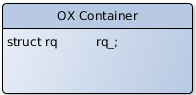
\includegraphics[width=0.5\textwidth]{images/oxc}
        \caption{Open-Extension Container}
        \label{fig:oxc}
\end{figure}
The ox container is designed as an abstract data structure; that is, any data
structure contains a \texttt{struct rq} runqueue inside can be called the ox
container. After bringing this new data structure into the kernel, there is 
not only per CPU runqueues in teh system now, but also per oxc runqueues.

\section{The oxc scheduling\label{sec:design_oxc_scheduling}}
As there are extra per oxc runqueues besides 
per CPU ones in a system, they can be candidates passed as parameters to 
scheduling operations. From the standpoint of a scheduler, it manages a task 
over the runqueue according to implementation details in the scheduling class, 
and as long as a runqueue parameter is provided for its scheduling operations, 
the scheduler does not care whether it is associated with a CPU or from an ox 
container. So, as a oxc local runqueue is passed to hooks of scheduling 
classes, \textbf{tasks would enqueue, operate and dequeue on a per container 
runqueue}. This is called \textbf{the oxc scheduling}. The task enqueued in
an ox container's local runqueue is called an oxc task. Of course, an oxc 
task can be a normal task or a rt task.

For tasks and scheduling classes, there is no difference between a per CPU 
and per container runqueue. This will be clearly shown when we see the 
scheduling route inside an ox container. 
Recall the path which relates each task with the per CPU runqueue it runs above.
Figure \ref{fig:cfs_scheme_tg} is the scheduling route for a task under 
cfs scheduling when fair task group scheduling is enabled; figure 
\ref{fig:rt_scheme_tg} is the shceduling route under rt scheduling when rt task 
group scheduling is enabled; figure \ref{fig:cfs_scheme_no_tg} is the 
scheduling route for a task without task group scheduling.
Now we are going to extend the scheduling routes in Linux for the oxc scheduling. 

It's very natural to merge oxc scheduling in Linux scheduling routes.
Figure \ref{fig:oxc_fair_tg} shows the extended sheduling route under cfs
scheduling with \texttt{CONFIG\_FAIR\_GROUP\_SCHED} enabled. The only
difference for an oxc task happens in the terminal, where a per ox container
runqueue replaces the per CPU counterpart. Figure \ref{fig:oxc_rt_tg} shows
the scheduling route under rt scheduling with \texttt{CONFIG\_RT\_GROUP\_SCHED}
enabled; the situation is similar to cfs scheduling case we just saw.
In fact, the scheduling route previous route can also lead a task to its per 
container runqueue. The same codes can still be used to find both kinds of 
runqueues.

\begin{figure}[htbp]
\begin{center}
	\subfigure[The route under cfs scheduling] {
        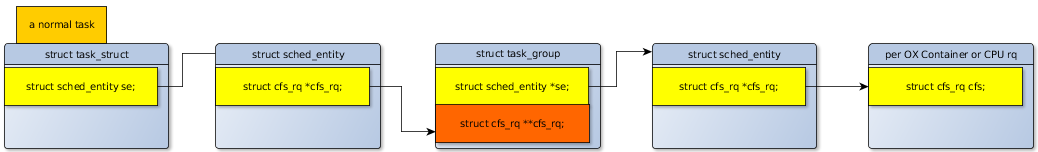
\includegraphics[height=2.5cm, width=\textwidth]{images/cfs_scheduling_scheme_tg_oxc}
        \label{fig:oxc_fair_tg}
	}
	\subfigure[The route under rt scheduling] {
        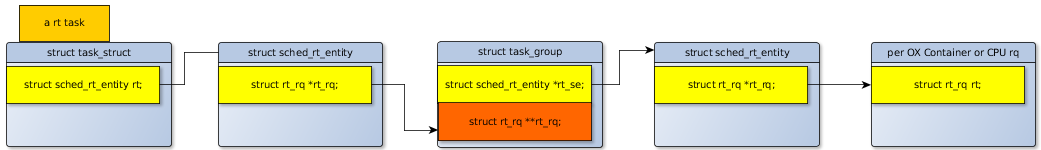
\includegraphics[height=2.5cm, width=\textwidth]{images/rt_scheduling_scheme_tg_oxc}
        \label{fig:oxc_rt_tg}
	}
\end{center}
	%\end{subfigure}
	\caption{Scheduling routes for a task with task group scheduling
			\\\indent\hspace{6cm} enabled }
	\label{fig:scheduling_route_oxc}
\end{figure}

In section \ref{sec:LinuxSched_cfs}, we introduce that when task group
scheduling is not enabled, a macro \texttt{task\_rq} is used to associate
a task to its runqueue. The \texttt{task\_rq} is defined as follows:
\begin{lstlisting}
#define task_rq(p)              cpu_rq(task_cpu(p))
\end{lstlisting}
The macro returns the associated rq for the CPU where the task is currently 
running on. So, when task group scheduling is not enabled, in order to merge
oxc scheduling in the system, a new path leading a task to a runqueue is 
needed, shown in figure \ref{fig:oxc_task_no_tg}. Actually, this path already 
exists in Linux kernel. Just because in mainline Linux, there is no runqueue 
other than per CPU ones and people ignore to exploit it.  
\begin{figure}[htbp]
        \centering
        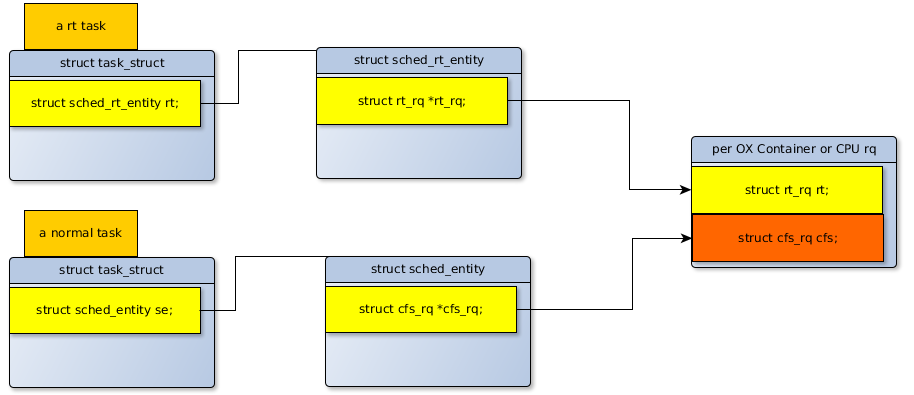
\includegraphics[width=\textwidth]{images/oxc_task_no_tg}
        \caption{New scheduling route for tasks when task group scheduling is \\
			\indent\hspace{6cm} not enabled}
        \label{fig:oxc_task_no_tg}
\end{figure}

The first feature of oxc scheduling is that it is compatibe with Linux original
scheduling design. Tasks dealt by rt scheduler or cfs can naturally work under the
oxc scheduling system. When there is new scheduling algorithm implemented in
Linux kernel, like the \emph{sched deadline} patch we mentioned before, the
new scheduler has to fullfill details behind scheduling interfaces in 
\texttt{struct sched\_class}. Again, for each shceduling class, they do not
care the interface is passed a per CPU or per container runqueue as the
parameter, and the new scheduling class can also work under oxc scheduling.
So, the ox container structure is open to extension; this is where the name
is from.

Based on per CPU scheduling, each scheduling operation defined in 
\texttt{struct sched\_class} will affect all tasks in the CPU. The
oxc scheduling provides another opportunity to apply a scheduling class in a 
fine grained scale. Now, the scale to apply a scheduler can be controlled 
in the unit of an ox container. 

\section{Movtivation for oxc scheduling framework}
In section \ref{sec:RelatedWork}, we see that, based on Linux, CPU bandwidth 
control can be applied in the level of single tasks or task groups which 
are shceudled by some policies. Such controls can be real-time or non real-time.
One obervation is that there does not exist a mechanism that can
control CPU bandwidth for all kinds of tasks as a whole without requirement of
a task' scheduling details. 

Suppose there is an ox container, different schedulers can use it to enqueue,
operate, and dequeue its tasks. If a fraction of CPU bandwidth can be assigned
to this ox container, all kinds of tasks will use it as running on a less powerful
machine. This is the oxc solution to the CPU bandwidth control for
general types of tasks.

Based on this idea, we develop an oxc scheduling framework in Linux that can 
realize multi processor CPU reservation for tasks without requiring scheduling
policies. 
%The oxc framework is not a scheduler. Although it cooperates with
%different scheduling classes, its pure responsibility is managing CPU power
%distribution. 
In the following chapter, details on how to implement 
this oxc scheduling framework in Linux kernel are described.
